\documentclass[landscape,a0paper,fontscale=0.285]{baposter} 

\usepackage{graphicx} 
\graphicspath{{figures/}}

\usepackage{amsmath} 
\usepackage{amssymb}

\usepackage{booktabs} 
\usepackage{enumitem} 
\usepackage{palatino} 
\usepackage[font=small,labelfont=bf]{caption} 

\usepackage{multicol} 
\setlength{\columnsep}{1.5em} 

\usepackage{tikz} 
\usetikzlibrary{shapes,arrows} 

\newcommand{\compresslist}{ 
\setlength{\itemsep}{1pt}
\setlength{\parskip}{0pt}
\setlength{\parsep}{0pt}
}

\definecolor{lightblue}{rgb}{0.145,0.6666,1} 

\begin{document}

\begin{poster}
{
headerborder=closed, 
colspacing=1em, 
bgColorOne=white, 
bgColorTwo=white,
borderColor=lightblue, 
headerColorOne=black, 
headerColorTwo=lightblue, 
headerFontColor=white, 
boxColorOne=white, 
textborder=roundedleft, 
eyecatcher=true, 
headerheight=0.1\textheight, 
headershape=roundedright, 
headerfont=\Large\bf\textsc, 
linewidth=2pt 
}
%----------------------------------------------------------------------------------------
%	Title 
%----------------------------------------------------------------------------------------
%
{
\includegraphics[height=11em]{NewcastleLogo.png}} 
{\bf\textsc{Very Cool Name}\vspace{0.5em}}
{\textsc{\{ Jack Tolhurst, Tory Jones, Naman Mor, James Harrison, and Edward Ma \} \newline University Of Newcastle}}
{
\includegraphics[height=11em]{NewcastleLogo.png}}

%----------------------------------------------------------------------------------------
%	Introduction
%----------------------------------------------------------------------------------------

\headerbox{Introduction}{name=introduction,column=0,row=0}{


Software Development is widespread across the IT field, with the sole purpose of controlling computers. The intention is to harness the resources of a computer system to provide useful functionality for the user or entity controlling said subject. Created by a developer, code can be written to take control of functionality that a computer has, and in unison, a device can be manipulated into performing tasks to reach an end goal. Software is used for many purposes, from controlling file systems, to games, to creative arts, to simply entertaining the user. However, when software is deployed in a specialized environment, this is a Specialized Software System. Specialized Software Systems are deployed for niche applications as opposed to broad applications, thus, they are often developed by specialized teams. For example, Microsoft Sharepoint has a Specialised Software System, in the form of a Database. Within a specific deployment, goals are easier to set, and developers can focus on features, algorithms, and implementations that may benefit the specific application over a generalized deployment. This may increase productivity of the host system, if optimized for the environment that a Specialized Software System is being deployed within.

}

%----------------------------------------------------------------------------------------
%	System Architecture
%----------------------------------------------------------------------------------------

\headerbox{System Architecture and Modelling}{name=SystemArchitecture,column=2,span=2,row=0}{

\begin{multicols}{2}
    Enterprise Information Management Systems (EIMS) rely on a structured system architecture emphasising  consistency, integration and scalability of data modelled across the strictly defined life cycle of information management (figure~\ref{fig:lifecycle}).  Information across its life cycle is first created before being classified through the use of metadata which declares information about the data based on type, source or sensitivity level \cite{verizon2023}.  Data is then stored into a tiered repository within the database in a location based on its access frequency or cruciality making it significantly easier to find with enterprise search tools. After data is Securely Stored within the database collaboration tools like Microsoft SharePoint are integrated into the EIMS to enable secure sharing over the internet while governance mechanisms ensure that data access is regulated within the system throughout its life cycle before its eventual disposition.
    
    
    \begin{center}
        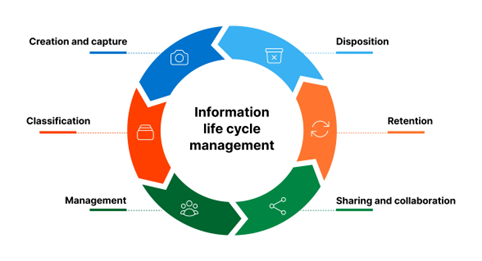
\includegraphics[width=0.8\linewidth]{InformationLifeCycle.png}
        \captionof{figure}{The Life Cycle of software development}
        \label{fig:lifecycle}
    \end{center}
\end{multicols}


}

%----------------------------------------------------------------------------------------
%	References
%----------------------------------------------------------------------------------------

\headerbox{References}{name=references,column=0,span=3,row=0.75,height=0.25}{

\renewcommand{\section}[2]{\vskip 0.05em}
\nocite{*} 
\small{ 
    \bibliographystyle{unsrt}
    \bibliography{bibliography}
}}

%----------------------------------------------------------------------------------------
%	Conclusion and Ethics
%----------------------------------------------------------------------------------------

\headerbox{Conclusion and Ethics}{name=conclusion,column=3,span=1,row=0,below=SystemArchitecture,above=bottom}{

In conclusion, Databases in Specialised Software Systems are everywhere. This is because, in many cases, commercial software may not be a viable solution to an issue. Especially in secure places like the aforementioned subjects where these systems may be deployed. However, there is now an ethical weakness. Specialised Software Systems can be developed indefinitely and will become astronomical in size. Take Microsoft Sharepoint, for example. So many people (or staff within the parent company) may be storing personal data on these systems, and therefore, may have a real-world damaging response to a data-breach. If these systems are accessible by third parties, they need to be built with the consideration of security. A large database with less-than-sufficient security is generally ethically dangerous. Though, large dedicated companies, such as those in the Defence area, may put way more emphasis on their security to protect internal data.

}

%----------------------------------------------------------------------------------------
%	DATA MANAGEMENT
%----------------------------------------------------------------------------------------

\headerbox{Data Management}{name=dataManagement,column=1,row=0,above=conclusion}{

Enterprise Information Management Systems (EIMS) structure how organisations manage data across its lifecycle: Create, Classify, Store, Retrieve, Share, and Govern. By integrating centralised repositories, metadata classification, and enterprise search, these systems reduce data fragmentation and improve accessibility \cite{armbrust2010}. Automated retrieval technologies can reduce document handling time by 40–50\%, significantly improving operational efficiency \cite{davenport2018}. However, large centralised repositories present significant security risks, becoming prime targets for cyberattacks and requiring robust data protection measures.
}

%----------------------------------------------------------------------------------------
%	Finance
%----------------------------------------------------------------------------------------

\headerbox{Finance}{name=finance,column=0,below=introduction,above=references}{

The following materials were required to complete the research:

\begin{itemize}\compresslist
\item Curabitur pellentesque dignissim
\item Eu facilisis est tempus quis
\item Duis porta consequat lorem
\item Eu facilisis est tempus quis
\end{itemize}

The following equations were used for statistical analysis:

\begin{equation}
\cos^3 \theta =\frac{1}{4}\cos\theta+\frac{3}{4}\cos 3\theta
\label{eq:refname}
\end{equation}\

}

%----------------------------------------------------------------------------------------
%	Defence Systems
%----------------------------------------------------------------------------------------

\headerbox{Defence Systems}{name=defence,column=1,below=SystemArchitecture,span=2,above=references}{ 
\begin{multicols}{2}
    The management of databases and their data within defence systems are inherent to national security and require state of the art software solutions. Interactions between countries and their national security follow security mandates set by international organisations, such as ISO 27001, which aim to continue 'establishing and continually improving… information security management systems' \cite{iso27001}. Another key concept for data management systems is implementing data-driven codebases that prioritise active control over functional-driven frameworks generally imposed upon databases. \cite{brynjolfsson2011}

    \columnbreak
    Social engineering attacks frequently pose a greater risk to defence operations as they are generally perceived as lower risk than generalised ones \cite{dataPlanning2015}. Hence, the Australian government, as of 2024, created the Cyber Security Act, where its main goal was to 'improve the response to and minimise the impact of cyber security incidents…' within society, while still giving governmental access to 'facilitate the whole of Government response to significant cyber security incidents…'\cite{cybersecurityAct2024}. This legislation also manages and secures sensitive data from perceived threats, providing citizens with a compliant software system that protects their data.

\end{multicols}


}

% --- end --- 

\end{poster}

\end{document}